\appendix
\section{Butcher Tableaus of the Fifth-Order Solvers}
\label{app:butcher}

A Butcher tableau lists the coefficients of Equation~\ref{eq:rk-general}:
the nodes $c_i$ (left column, the fraction of the step at which stage $i$ is
evaluated), the stage weights $a_{ij}$ (lower triangle) and the solution
weights $b_i$ (bottom row). Tables~\ref{tab:butcher-dopri5}
and~\ref{tab:butcher-tsit5} list the two fifth-order methods used in this
report. Both have seven stages with
$b_7=0$; the seventh stage exists only for the embedded error estimate and
is skipped by this project's fixed-step integrator, so each costs six field
evaluations per step. Coefficients are the ones used in this project's code
(DOPRI5 exact, Tsit5 to the precision given in \cite{tsitouras2011tsit5},
shown here to six decimals).

\begin{table}[!ht]
\centering
\footnotesize
\renewcommand{\arraystretch}{1.25}
\caption{DOPRI5 \cite{dormand1980dopri}, fifth-order solution weights.}
\label{tab:butcher-dopri5}
$\begin{array}{c|ccccccc}
0 \\
\tfrac15 & \tfrac15\\
\tfrac{3}{10} & \tfrac{3}{40} & \tfrac{9}{40}\\
\tfrac45 & \tfrac{44}{45} & -\tfrac{56}{15} & \tfrac{32}{9}\\
\tfrac89 & \tfrac{19372}{6561} & -\tfrac{25360}{2187} & \tfrac{64448}{6561} & -\tfrac{212}{729}\\
1 & \tfrac{9017}{3168} & -\tfrac{355}{33} & \tfrac{46732}{5247} & \tfrac{49}{176} & -\tfrac{5103}{18656}\\
1 & \tfrac{35}{384} & 0 & \tfrac{500}{1113} & \tfrac{125}{192} & -\tfrac{2187}{6784} & \tfrac{11}{84}\\
\hline
b & \tfrac{35}{384} & 0 & \tfrac{500}{1113} & \tfrac{125}{192} & -\tfrac{2187}{6784} & \tfrac{11}{84} & 0
\end{array}$
\end{table}

\begin{table}[!ht]
\centering
\footnotesize
\renewcommand{\arraystretch}{1.25}
\caption{Tsit5 \cite{tsitouras2011tsit5}, fifth-order solution weights.}
\label{tab:butcher-tsit5}
\resizebox{\textwidth}{!}{%
$\begin{array}{c|ccccccc}
0 \\
0.161 & 0.161\\
0.327 & -0.008481 & 0.335481\\
0.9 & 2.897153 & -6.359448 & 4.362295\\
0.980026 & 5.325865 & -11.748884 & 7.495539 & -0.092495\\
1 & 5.861455 & -12.920969 & 8.159368 & -0.071585 & -0.028269\\
1 & 0.096461 & 0.01 & 0.479890 & 1.379009 & -3.290070 & 2.324711\\
\hline
b & 0.096461 & 0.01 & 0.479890 & 1.379009 & -3.290070 & 2.324711 & 0
\end{array}$}
\end{table}

In both tableaus the last row of $a_{ij}$ equals $b$: the final stage is
evaluated at the new solution itself (``first same as last''), which is what
makes it free to reuse as the next step's first stage in an adaptive solver.
The solution weights sum to one in both cases, the first of the order
conditions, and this is one of the automated checks
(Section~\ref{sec:verification}).

\clearpage
\section{Damping-Study Trajectories}
\label{app:stiffness-figs}

The two figures below expand the trajectory comparison of
Section~\ref{sec:track-d} at full page width. In each, the top row shows the
predicted angle $\theta(t)$ and angular velocity $\omega(t)$ of every
solver's model next to the true trajectory, the bottom left shows the
magnitude of each solver's own learned field $|\mathbf f_\theta|$ over
$(\theta,\omega)$ with that model's trajectory drawn on it, and the bottom
right shows the logarithm of the pointwise error. Legends give each model's
verdict under the rule of Section~\ref{sec:track-d}. The trajectories were
recomputed from the saved seed-42 checkpoints, and each reproduces its
recorded best training MSE.

\begin{figure}[htbp]
\centering
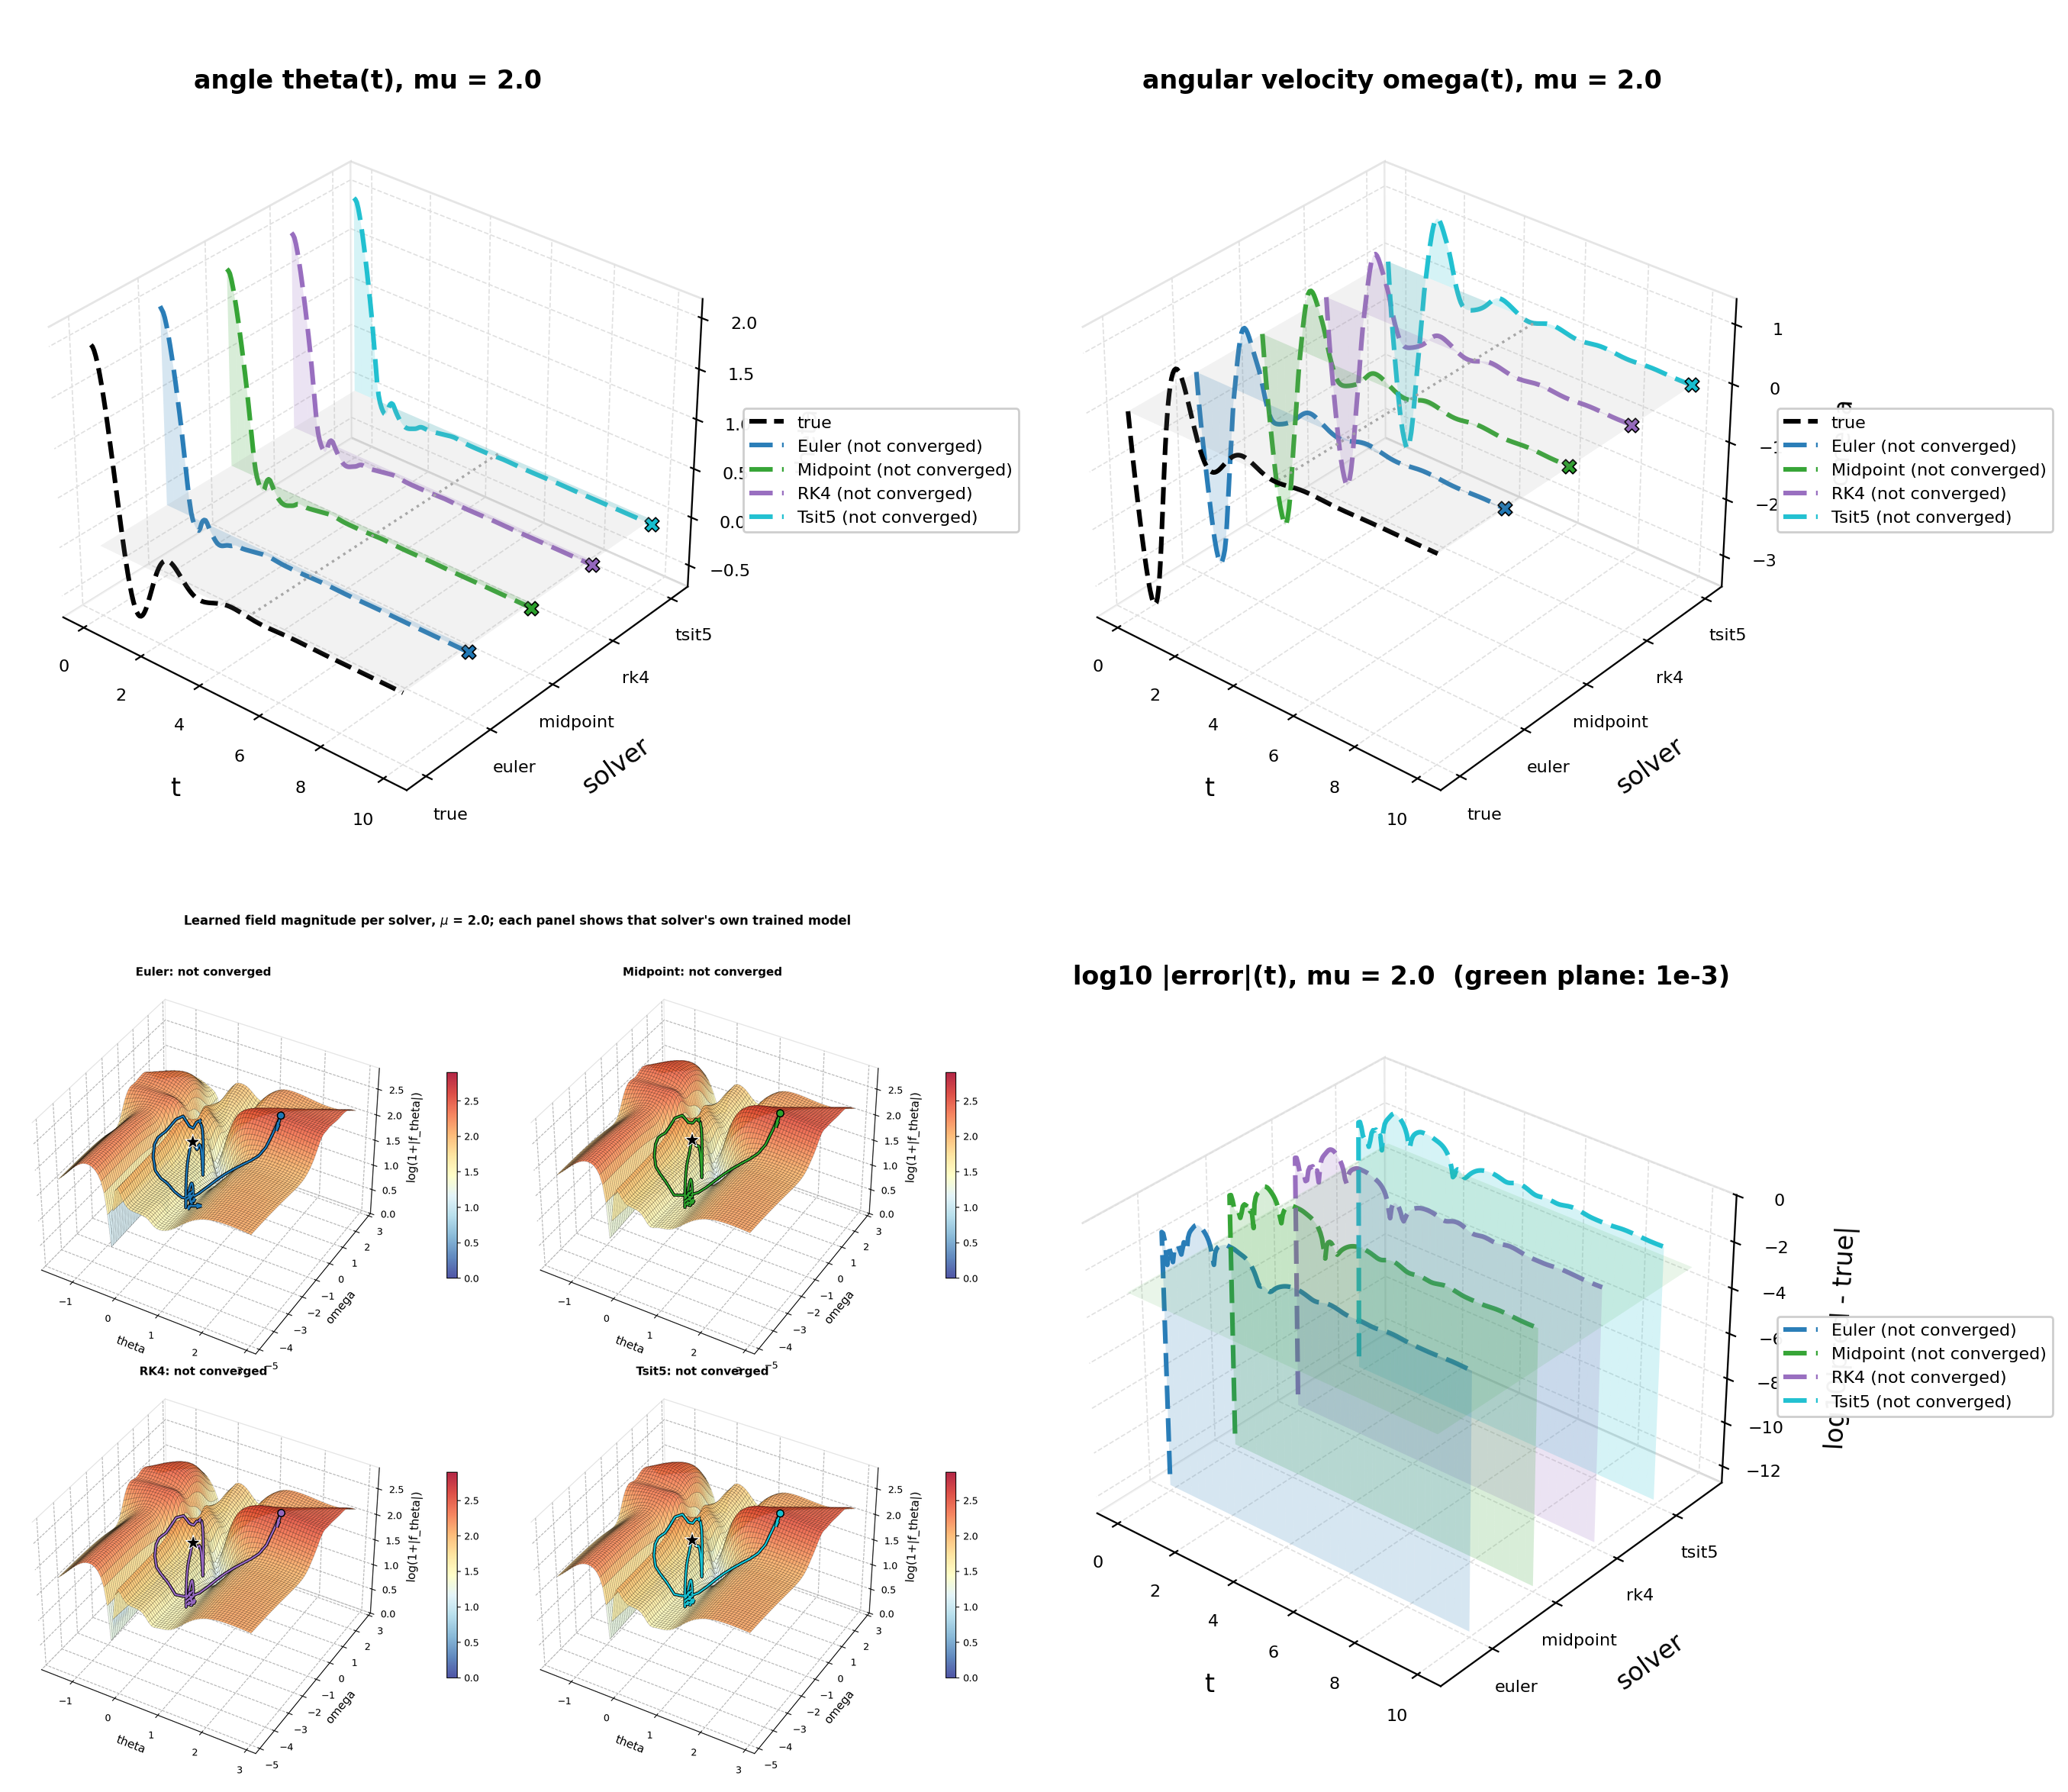
\includegraphics[width=\textwidth]{figures/track_d/mu2.0_trajectory_grid.png}
\caption{$\mu=2.0$, all four solvers (seed 42). Every model settles onto the
same wrong trajectory, which ends at the learned spurious equilibrium of
Table~\ref{tab:spurious-eq}.}
\label{fig:mu2-collage}
\end{figure}

\begin{figure}[htbp]
\centering
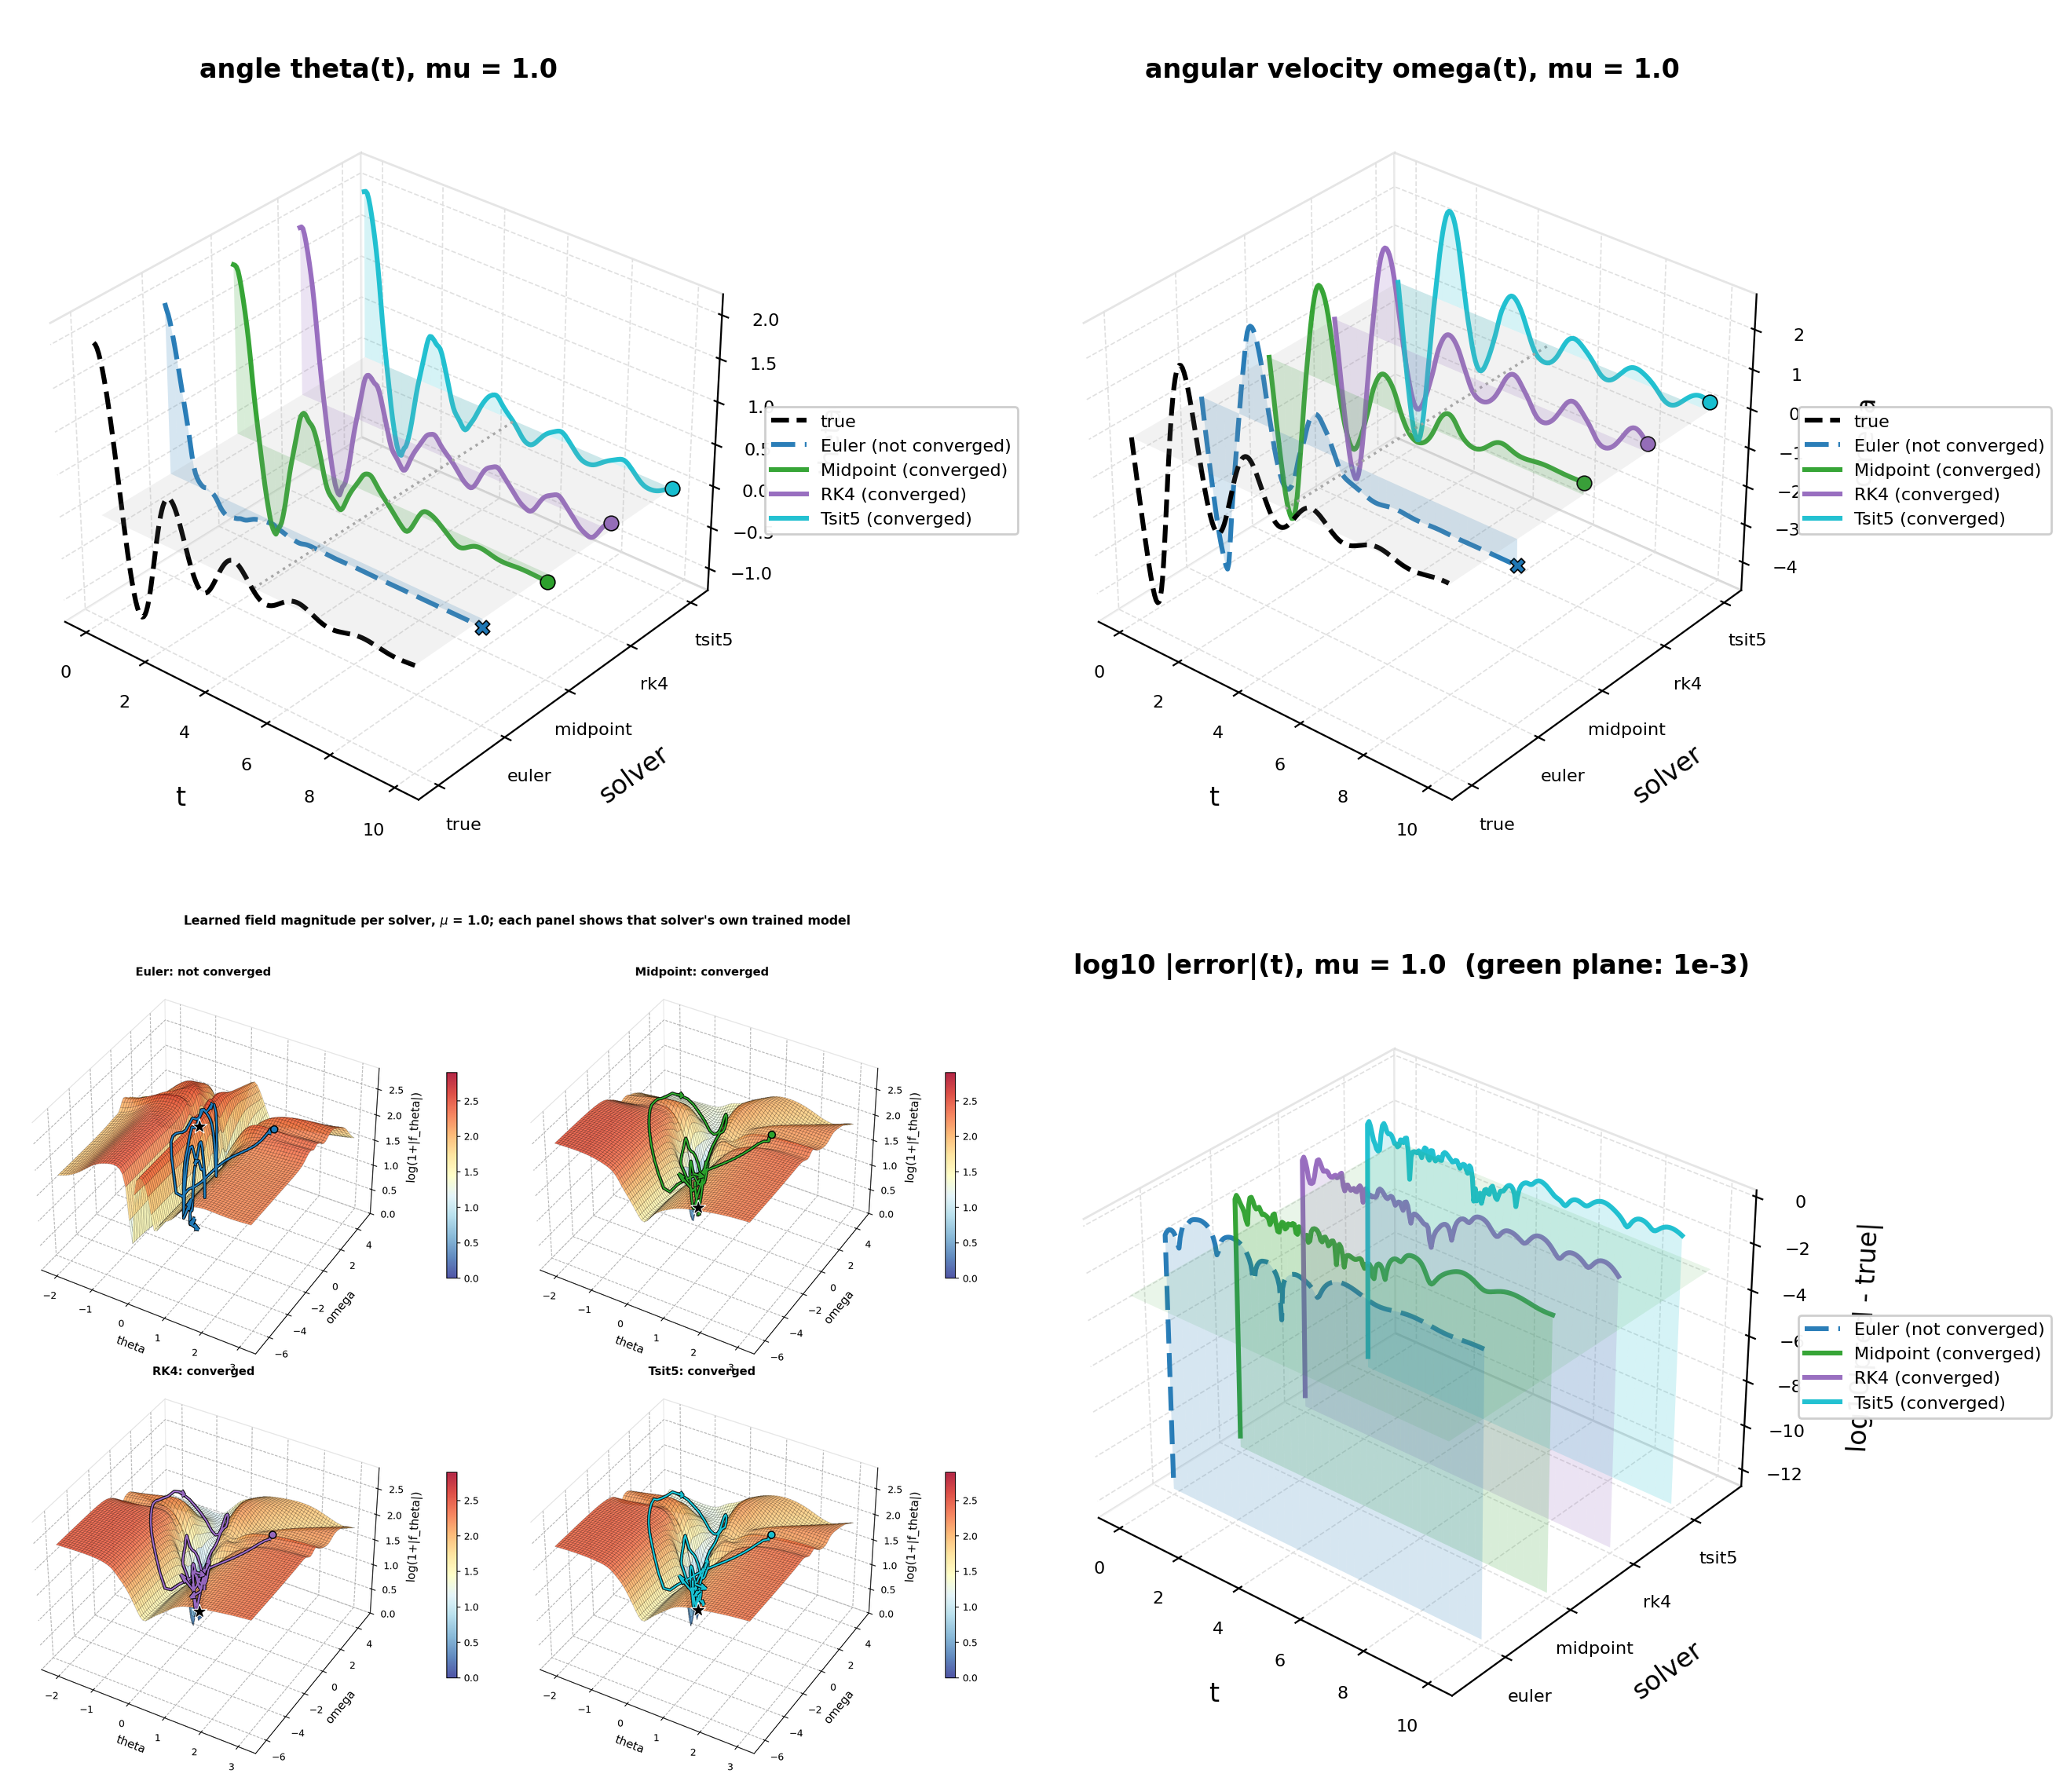
\includegraphics[width=\textwidth]{figures/track_d/mu1.0_trajectory_grid.png}
\caption{$\mu=1.0$, all four solvers (seed 42), in the same layout. Only
Euler's predicted angle departs visibly from the true one; the other three
track it closely.}
\label{fig:mu1-collage}
\end{figure}
